% SPDX-FileCopyrightText: © 2026 Idiap Research Institute <contact@idiap.ch>
%
% SPDX-FileContributor: Andre Freitas <andre.freitas@idiap.ch>
% Neuro-symbolic AI Group
%
% SPDX-FileContributor: Danilo Gusicuma <danilo.gusicuma@idiap.ch>
% Neuro-symbolic AI Group
%
% SPDX-License-Identifier: MIT
\section{Native workflow composition}
\label{app:native-workflow}
This bounded example describes the native declaration of \texttt{abducer\_work\_loop}.
Its typed boundaries preserve generated wrappers and the derived claim needed by calibration.
Write $G,H,C,V,J,S$ for gap, hypothesis, derived claim, assessment, routing input,
and routing assessment, and $\operatorname{Gen}[T]$ for the literal generated wrapper.
The record boundary $B$ contains a claim of type $C$ and an assessment of type
$\operatorname{Gen}[V]$. This notation supplies no product universal property.
\[
\begin{aligned}
G&\xrightarrow{a}\operatorname{Gen}[H]\xrightarrow{u_h}H
\xrightarrow{d}\operatorname{Gen}[C]\xrightarrow{u_c}C\\
&\xrightarrow{r_{\mathrm{ctx}}}B\xrightarrow{p}J\xrightarrow{e}\operatorname{Gen}[S].
\end{aligned}
\]
Here $r_{\mathrm{ctx}}$ models the refutation occurrence with its existing claim
binding retained; $p$ constructs the two-field routing input and unwraps the assessment.
The displayed arrows generate a free path category: identities are empty paths and
composition concatenates matching paths. This is a syntactic construction.
The original source separately declares release, reframe, retarget, and refuted-stop routing;
the native declaration returns an assessment without executing those branches.
No execution, semantic equivalence, monad structure, or scientific truth follows.

The projections $u_h,u_c$ and the assessment projection in $p$ refer to payloads of successfully obtained generated results. They do not remove a model failure or establish the truth of generated content. The construction describes one native interface; it does not reconstruct every canonical workflow.
\begin{figure}[htbp]
\centering
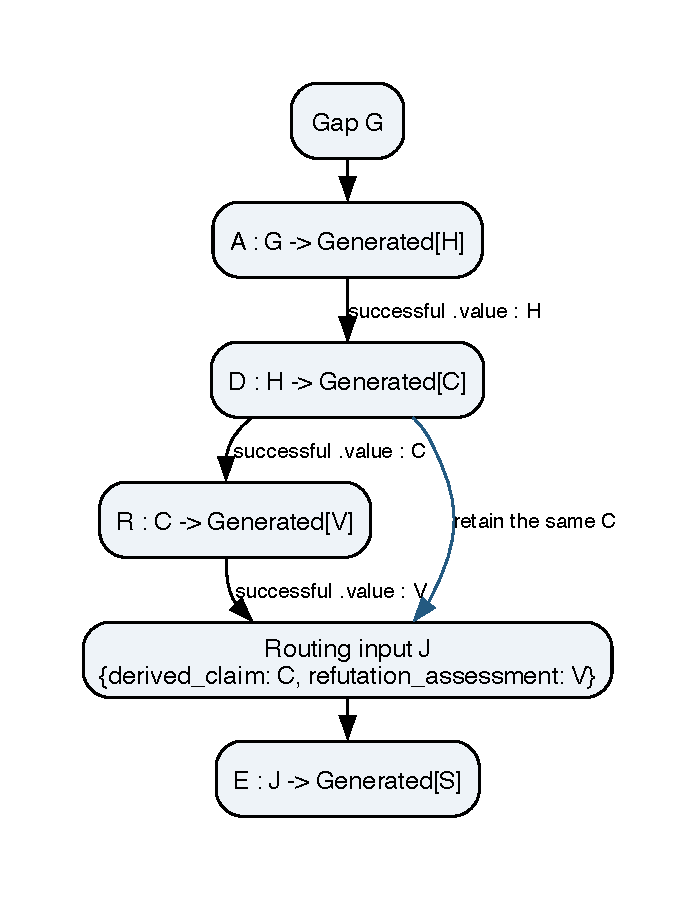
\includegraphics[width=.85\linewidth,height=.56\textheight,keepaspectratio]{paper-workflow-representations/native-interfaces.pdf}
\caption{Native input/output boundaries of the local abductive workflow. $G,H,C,V,J,S$ are nominal payload types, not a subtype hierarchy. Every occurrence produces a generated wrapper; calibration consumes a record containing the same claim tested by refutation and its assessment. Materialized failures are outside this successful-result view.}
\label{fig:native-interfaces}
\end{figure}

\section{Claim-indexed workflow interfaces}
\label{app:dependent-workflow}
The native \texttt{abducer\_work\_loop} keeps both a derived claim and its
refutation assessment when constructing the routing input. Its assessment type
is nominal: the native declaration does not encode which claim was assessed
in the type. We propose the following dependent-type-style presentation as a
paper-level refinement of that interface. It adds an exact input association
for exposition; it does not report a dependent-type implementation or a
machine-checked proof. Existing epistemic handles and reasoning occurrences
retain their meaning.

\paragraph{Claim-indexed assessment.}
Let $\mathsf{Claim}$ and $\mathsf{NativeAssessment}$ name the corresponding
native payload types. In the proposed presentation, an indexed assessment is
a record of an assessment occurrence associated with its exact input claim.
With a stipulated provenance-record family $\mathsf{Linked}(c,v)$, define $\mathsf{Assessment}(c):=\sum_{v:\mathsf{NativeAssessment}}\mathsf{Linked}(c,v)$. Its producer remains an unresolved realization obligation. We declare its formation and forgetting map:
\[
 c:\mathsf{Claim}\vdash\mathsf{Assessment}(c)\;\mathsf{type},\qquad
 \mathsf{erase}_c:\mathsf{Assessment}(c)\to\mathsf{NativeAssessment}.
\]
The stipulated linkage-record contract is indexed by its input claim. Thus an assessment associated
with $c_1$ cannot be supplied at $c_2$ merely because both claims have the same
nominal type. This association records the target of an assessment, not its
truth, adequacy, or correctness. The model does not provide a promotion from
an arbitrary native payload to a scientifically warranted assessment.

The dependent pair retains exactly the context needed by calibration:
\[
 \mathsf{RoutingInput}^{\star}
   :=\sum_{c:\mathsf{Claim}}\mathsf{Assessment}(c),\qquad
 \frac{\Gamma\vdash c:\mathsf{Claim}\quad
       \Gamma\vdash a:\mathsf{Assessment}(c)}
      {\Gamma\vdash(c,a):\mathsf{RoutingInput}^{\star}}.
\]
Erasing $(c,a)$ gives the native record
$\texttt{derived\_claim}=c$ and
$\texttt{refutation\_assessment}=\mathsf{erase}_c(a)$.
The family expresses a restriction that an ordinary pair of independently
chosen native values cannot express. This erasure is a proposed correspondence;
no general equivalence of type systems is asserted.

\paragraph{Operations and retained context.}
The proposed refutation interface is
\[
 \mathsf{assess}^{\star}:\prod_{c:\mathsf{Claim}}
             \mathsf{Generated}[\mathsf{Assessment}(c)].
\]
\[
 \mathsf{calibrate}^{\star}:\mathsf{RoutingInput}^{\star}\to
             \mathsf{Generated}[\mathsf{RoutingAssessment}].
\]
Application substitutes the actual claim for the binder:
$\mathsf{assess}^{\star}(c_1):
\mathsf{Generated}[\mathsf{Assessment}(c_1)]$.
Under an explicitly proposed value accessor for this new indexed payload, after a successfully obtained generated result,
the context is
$\Gamma,c_1:\mathsf{Claim},a_1:\mathsf{Assessment}(c_1)$.
The native source uses \texttt{derived\_claim.value} both for the assessment
input and for the subsequent routing record. This source binding motivates
the refined association. The materialized agents have the separate interface
$\mathsf{Result}[\mathsf{Generated}[T],\mathsf{ModelFailure}]$ and declared
\texttt{AI.Generate} and \texttt{Context.Disclose} effects. The display above
is a successful-result interface, not a claim of total execution or a law
permitting all generated results to be unwrapped unconditionally.

\paragraph{Substitution and equality boundaries.}
For $\Delta=(c:\mathsf{Claim},a:\mathsf{Assessment}(c))$, a substitution
$\sigma:\Gamma\to\Delta$ must supply $c_1:\mathsf{Claim}$ and
$a_1:\mathsf{Assessment}(c_1)$ together. It is invalid to replace the first
binding by $c_2$ while retaining $a_1$ at the old index. Binder renaming and
capture-avoiding substitution are presentation rules. If an identity type is
assumed and an explicit witness
$p:\mathsf{Id}_{\mathsf{Claim}}(c_1,c_2)$ is supplied, a separately declared
transport operation has type
\[
 \mathsf{transport}_{\mathsf{Assessment}}(p,-):
 \mathsf{Assessment}(c_1)\to\mathsf{Assessment}(c_2).
\]
This conditional rule is not an assertion that such a witness exists.
Matching labels, similar prose, source hashes, and empirical agreement provide
no identity witness. Definitional conversion is limited to the declared
syntactic rules; it is not an empirical equivalence judgment.

\paragraph{Epistemic and control limits.}
A term of $\mathsf{Generated}[T]$ represents generated content. Neither that
wrapper nor a native relation record supplies a proof of the content's
proposition. In particular, a routing assessment containing
\texttt{ReadyForReleasePromotion} does not execute a release. The original
workflow's release, reframe, retarget, and refuted-stop clauses remain original
layer policy annotations. This bounded description asserts no termination,
normalization, univalence, runtime dependent-type enforcement, or scientific
success. Its benefit as notation is specific: the claim required by the final
join stays visible, and an assessment of another claim cannot silently replace
its dependent partner.

\paragraph{A concrete index mismatch.}
In the diffusion example, let $c_{\mathrm{fixed}}$ state exponential decay for one fixed connected graph and $c_{\mathrm{uniform}}$ state a common positive decay rate for all connected graphs. An assessment of the cycle-family counterexample belongs to the latter claim. Pairing it with the former would change what was tested. The indexed interface exposes this mismatch: an element of $\mathsf{Assessment}(c_{\mathrm{uniform}})$ cannot be reused at $c_{\mathrm{fixed}}$ without an applicable definitional equality or an explicit identity witness and transport. No such identification is provided here. Calibration must instead retain the two distinct statements and explain why only the uniform strengthening fails.


\clearpage
\section{Reasoning taxonomy and artifact roles}
\label{app:reasoning-taxonomy}
Figure~\ref{fig:reasoning-taxonomy} summarizes the eight primitive reasoning families used in the main text. Dashed links express functional membership, not temporal order, exclusive classification, or subtyping. These layers can overlap in a larger inquiry; this figure shows their organizing roles. Figure~\ref{fig:native-interfaces} separately shows concrete native types and data dependencies for one workflow. The distinction matters: a conceptual taxonomy does not determine an executable signature.
\begin{figure}[htbp]
\centering
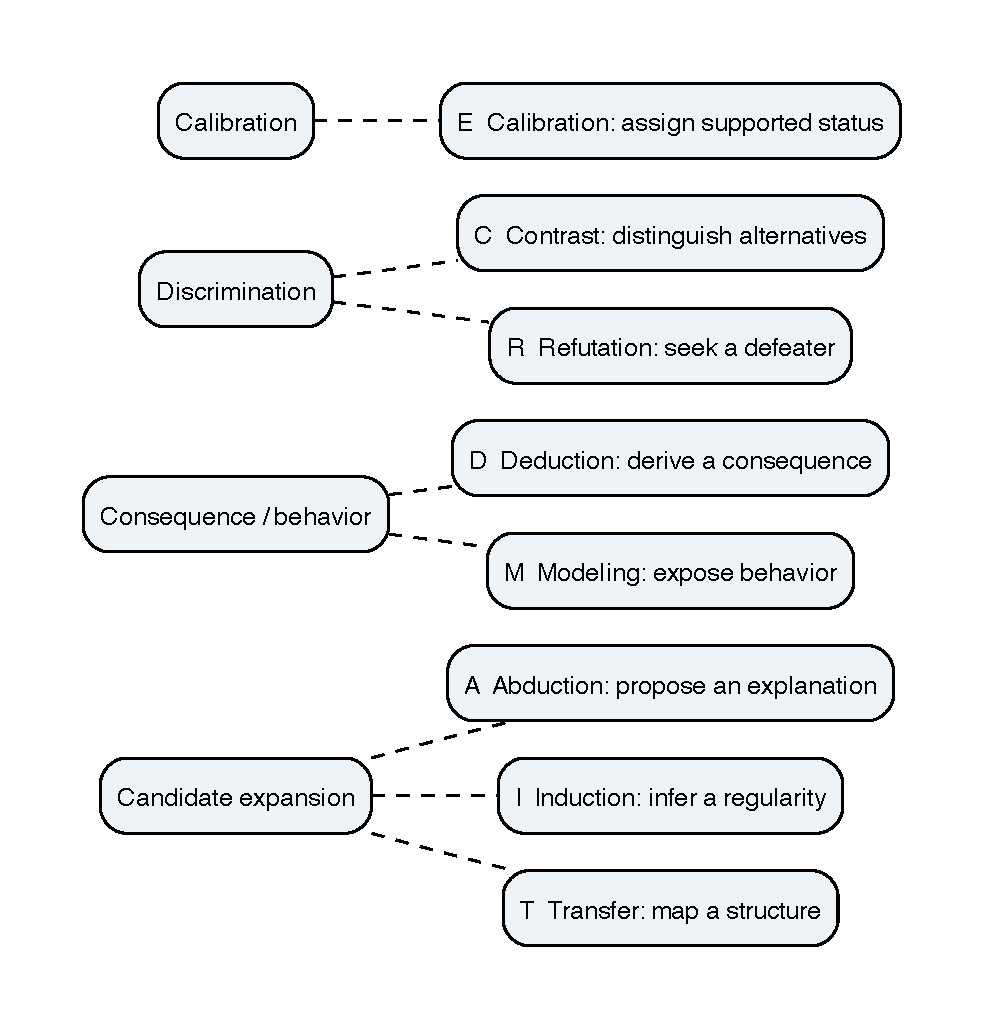
\includegraphics[width=\linewidth,height=.47\textheight,keepaspectratio]{paper-workflow-representations/reasoning-taxonomy.pdf}
\caption{Functional taxonomy of reasoning. Candidate creation, consequence exposure, discrimination, and calibration have distinct responsibilities. The links classify the displayed roles; they are not execution arrows.}
\label{fig:reasoning-taxonomy}
\end{figure}

\begin{center}
\small
\begin{tabularx}{\linewidth}{@{}lXX@{}}
\toprule
Mechanism & Typical input role & Typical output role \\
\midrule
Abduction & Gap and constraints & Candidate explanation or premise \\
Induction & Observations under a scope & Proposed regularity \\
Transfer & Source structure and target constraints & Proposed bridge with obligations \\
Deduction & Explicit premises & Scoped consequence \\
Modeling & Model and conditions & Predicted or simulated behavior \\
Contrast & Alternatives and discriminating question & Relevant difference \\
Refutation & Claim and critical test & Defeater or bounded test outcome \\
Calibration & Retained claim, evidence and context & Supported status and remaining obligations \\
\bottomrule
\end{tabularx}
\end{center}
These are explanatory artifact roles, not additional native type declarations. A model output or assessment may be mistaken; well-matched inputs alone do not supply scientific warrant.
